% Options for packages loaded elsewhere
\PassOptionsToPackage{unicode}{hyperref}
\PassOptionsToPackage{hyphens}{url}
%
\documentclass[
]{book}
\usepackage{amsmath,amssymb}
\usepackage{iftex}
\ifPDFTeX
  \usepackage[T1]{fontenc}
  \usepackage[utf8]{inputenc}
  \usepackage{textcomp} % provide euro and other symbols
\else % if luatex or xetex
  \usepackage{unicode-math} % this also loads fontspec
  \defaultfontfeatures{Scale=MatchLowercase}
  \defaultfontfeatures[\rmfamily]{Ligatures=TeX,Scale=1}
\fi
\usepackage{lmodern}
\ifPDFTeX\else
  % xetex/luatex font selection
\fi
% Use upquote if available, for straight quotes in verbatim environments
\IfFileExists{upquote.sty}{\usepackage{upquote}}{}
\IfFileExists{microtype.sty}{% use microtype if available
  \usepackage[]{microtype}
  \UseMicrotypeSet[protrusion]{basicmath} % disable protrusion for tt fonts
}{}
\makeatletter
\@ifundefined{KOMAClassName}{% if non-KOMA class
  \IfFileExists{parskip.sty}{%
    \usepackage{parskip}
  }{% else
    \setlength{\parindent}{0pt}
    \setlength{\parskip}{6pt plus 2pt minus 1pt}}
}{% if KOMA class
  \KOMAoptions{parskip=half}}
\makeatother
\usepackage{xcolor}
\usepackage{color}
\usepackage{fancyvrb}
\newcommand{\VerbBar}{|}
\newcommand{\VERB}{\Verb[commandchars=\\\{\}]}
\DefineVerbatimEnvironment{Highlighting}{Verbatim}{commandchars=\\\{\}}
% Add ',fontsize=\small' for more characters per line
\usepackage{framed}
\definecolor{shadecolor}{RGB}{248,248,248}
\newenvironment{Shaded}{\begin{snugshade}}{\end{snugshade}}
\newcommand{\AlertTok}[1]{\textcolor[rgb]{0.94,0.16,0.16}{#1}}
\newcommand{\AnnotationTok}[1]{\textcolor[rgb]{0.56,0.35,0.01}{\textbf{\textit{#1}}}}
\newcommand{\AttributeTok}[1]{\textcolor[rgb]{0.13,0.29,0.53}{#1}}
\newcommand{\BaseNTok}[1]{\textcolor[rgb]{0.00,0.00,0.81}{#1}}
\newcommand{\BuiltInTok}[1]{#1}
\newcommand{\CharTok}[1]{\textcolor[rgb]{0.31,0.60,0.02}{#1}}
\newcommand{\CommentTok}[1]{\textcolor[rgb]{0.56,0.35,0.01}{\textit{#1}}}
\newcommand{\CommentVarTok}[1]{\textcolor[rgb]{0.56,0.35,0.01}{\textbf{\textit{#1}}}}
\newcommand{\ConstantTok}[1]{\textcolor[rgb]{0.56,0.35,0.01}{#1}}
\newcommand{\ControlFlowTok}[1]{\textcolor[rgb]{0.13,0.29,0.53}{\textbf{#1}}}
\newcommand{\DataTypeTok}[1]{\textcolor[rgb]{0.13,0.29,0.53}{#1}}
\newcommand{\DecValTok}[1]{\textcolor[rgb]{0.00,0.00,0.81}{#1}}
\newcommand{\DocumentationTok}[1]{\textcolor[rgb]{0.56,0.35,0.01}{\textbf{\textit{#1}}}}
\newcommand{\ErrorTok}[1]{\textcolor[rgb]{0.64,0.00,0.00}{\textbf{#1}}}
\newcommand{\ExtensionTok}[1]{#1}
\newcommand{\FloatTok}[1]{\textcolor[rgb]{0.00,0.00,0.81}{#1}}
\newcommand{\FunctionTok}[1]{\textcolor[rgb]{0.13,0.29,0.53}{\textbf{#1}}}
\newcommand{\ImportTok}[1]{#1}
\newcommand{\InformationTok}[1]{\textcolor[rgb]{0.56,0.35,0.01}{\textbf{\textit{#1}}}}
\newcommand{\KeywordTok}[1]{\textcolor[rgb]{0.13,0.29,0.53}{\textbf{#1}}}
\newcommand{\NormalTok}[1]{#1}
\newcommand{\OperatorTok}[1]{\textcolor[rgb]{0.81,0.36,0.00}{\textbf{#1}}}
\newcommand{\OtherTok}[1]{\textcolor[rgb]{0.56,0.35,0.01}{#1}}
\newcommand{\PreprocessorTok}[1]{\textcolor[rgb]{0.56,0.35,0.01}{\textit{#1}}}
\newcommand{\RegionMarkerTok}[1]{#1}
\newcommand{\SpecialCharTok}[1]{\textcolor[rgb]{0.81,0.36,0.00}{\textbf{#1}}}
\newcommand{\SpecialStringTok}[1]{\textcolor[rgb]{0.31,0.60,0.02}{#1}}
\newcommand{\StringTok}[1]{\textcolor[rgb]{0.31,0.60,0.02}{#1}}
\newcommand{\VariableTok}[1]{\textcolor[rgb]{0.00,0.00,0.00}{#1}}
\newcommand{\VerbatimStringTok}[1]{\textcolor[rgb]{0.31,0.60,0.02}{#1}}
\newcommand{\WarningTok}[1]{\textcolor[rgb]{0.56,0.35,0.01}{\textbf{\textit{#1}}}}
\usepackage{longtable,booktabs,array}
\usepackage{calc} % for calculating minipage widths
% Correct order of tables after \paragraph or \subparagraph
\usepackage{etoolbox}
\makeatletter
\patchcmd\longtable{\par}{\if@noskipsec\mbox{}\fi\par}{}{}
\makeatother
% Allow footnotes in longtable head/foot
\IfFileExists{footnotehyper.sty}{\usepackage{footnotehyper}}{\usepackage{footnote}}
\makesavenoteenv{longtable}
\usepackage{graphicx}
\makeatletter
\def\maxwidth{\ifdim\Gin@nat@width>\linewidth\linewidth\else\Gin@nat@width\fi}
\def\maxheight{\ifdim\Gin@nat@height>\textheight\textheight\else\Gin@nat@height\fi}
\makeatother
% Scale images if necessary, so that they will not overflow the page
% margins by default, and it is still possible to overwrite the defaults
% using explicit options in \includegraphics[width, height, ...]{}
\setkeys{Gin}{width=\maxwidth,height=\maxheight,keepaspectratio}
% Set default figure placement to htbp
\makeatletter
\def\fps@figure{htbp}
\makeatother
\setlength{\emergencystretch}{3em} % prevent overfull lines
\providecommand{\tightlist}{%
  \setlength{\itemsep}{0pt}\setlength{\parskip}{0pt}}
\setcounter{secnumdepth}{5}
\usepackage{booktabs}
\usepackage{amsthm}
\makeatletter
\def\thm@space@setup{%
  \thm@preskip=8pt plus 2pt minus 4pt
  \thm@postskip=\thm@preskip
}
\makeatother
\ifLuaTeX
  \usepackage{selnolig}  % disable illegal ligatures
\fi
\usepackage[]{natbib}
\bibliographystyle{apalike}
\IfFileExists{bookmark.sty}{\usepackage{bookmark}}{\usepackage{hyperref}}
\IfFileExists{xurl.sty}{\usepackage{xurl}}{} % add URL line breaks if available
\urlstyle{same}
\hypersetup{
  pdftitle={MODELACIÓN DEL PRECIO PARA LA COMPRA Y VENTA DE ACEITE DE SOYA},
  pdfauthor={Nidia Munevar - Leonardo Palacios},
  hidelinks,
  pdfcreator={LaTeX via pandoc}}

\title{MODELACIÓN DEL PRECIO PARA LA COMPRA Y VENTA DE ACEITE DE SOYA}
\author{Nidia Munevar - Leonardo Palacios}
\date{2023-08-21}

\begin{document}
\maketitle

{
\setcounter{tocdepth}{1}
\tableofcontents
}
\hypertarget{resumen}{%
\chapter{Resumen}\label{resumen}}

El proyecto aplicado a realizar es la modelación del precio para la compra y venta de aceite de soya.

\hypertarget{introduccion}{%
\chapter{Introduccion}\label{introduccion}}

En el mercado de venta y compra de materias primas agrícolas intervienen diferentes actores, los precios son públicos y son afectados por diferentes variables tales como el precio del petróleo, la tasa de cambio, el clima entre otros elementos. La necesidad de los actores es mejorar sus decisiones y de esta forma su rentabilidad, los precios de las materias primas afectan directamente al mercado y a los precios de los bienes producidos a partir de estas, es decir estos valores terminan impactando al comprador final.

\hypertarget{justificacion}{%
\chapter{Justificacion}\label{justificacion}}

El proyecto está planteado ante una necesidad de los actores que requieren mejorar sus decisiones y de esta forma su rentabilidad. Los precios de las materias primas afectan directamente al mercado y a los precios de los bienes producidos a partir de estas materias, es decir estos valores terminan impactando al comprador final.

\hypertarget{serie-de-tiempo}{%
\chapter{Serie de Tiempo}\label{serie-de-tiempo}}

\begin{Shaded}
\begin{Highlighting}[]
\CommentTok{\# Instalar y cargar las librerías necesarias}
\CommentTok{\#install.packages("quantmod")}
\FunctionTok{library}\NormalTok{(quantmod)}
\end{Highlighting}
\end{Shaded}

\begin{verbatim}
## Loading required package: xts
\end{verbatim}

\begin{verbatim}
## Loading required package: zoo
\end{verbatim}

\begin{verbatim}
## 
## Attaching package: 'zoo'
\end{verbatim}

\begin{verbatim}
## The following objects are masked from 'package:base':
## 
##     as.Date, as.Date.numeric
\end{verbatim}

\begin{verbatim}
## Loading required package: TTR
\end{verbatim}

\begin{verbatim}
## Registered S3 method overwritten by 'quantmod':
##   method            from
##   as.zoo.data.frame zoo
\end{verbatim}

\begin{Shaded}
\begin{Highlighting}[]
\CommentTok{\# Simbolo del aceite de soya en Yahoo Finance}
\NormalTok{company }\OtherTok{\textless{}{-}} \StringTok{\textquotesingle{}ZS=F\textquotesingle{}}

\CommentTok{\# Definir fecha de inicio y del día de hoy}
\NormalTok{start }\OtherTok{\textless{}{-}} \FunctionTok{as.Date}\NormalTok{(}\StringTok{"2010{-}01{-}01"}\NormalTok{)}
\NormalTok{today }\OtherTok{\textless{}{-}} \FunctionTok{Sys.Date}\NormalTok{()}

\CommentTok{\# Conexión a Yahoo Finance para descargar la información}
\NormalTok{df }\OtherTok{\textless{}{-}} \FunctionTok{getSymbols}\NormalTok{(company, }\AttributeTok{src =} \StringTok{"yahoo"}\NormalTok{, }\AttributeTok{from =}\NormalTok{ start, }\AttributeTok{to =}\NormalTok{ today, }\AttributeTok{auto.assign =} \ConstantTok{FALSE}\NormalTok{)}

\CommentTok{\# Visualizar información de las últimas filas}
\FunctionTok{tail}\NormalTok{(df, }\DecValTok{10}\NormalTok{)}
\end{Highlighting}
\end{Shaded}

\begin{verbatim}
##            ZS=F.Open ZS=F.High ZS=F.Low ZS=F.Close ZS=F.Volume ZS=F.Adjusted
## 2023-08-07   1430.00   1430.00  1405.00    1414.50         212       1414.50
## 2023-08-08   1400.25   1431.25  1395.00    1430.00         382       1430.00
## 2023-08-09   1436.00   1438.00  1430.75    1431.50         104       1431.50
## 2023-08-10   1431.75   1438.50  1410.00    1412.00          82       1412.00
## 2023-08-11   1353.25   1409.00  1353.25    1401.25          25       1401.25
## 2023-08-14   1422.00   1422.00  1391.00    1391.00        7906       1391.00
## 2023-08-15   1344.25   1348.75  1319.50    1323.25       15884       1323.25
## 2023-08-16   1323.75   1344.25  1321.25    1334.75        9256       1334.75
## 2023-08-17   1337.00   1347.75  1332.50    1336.75       12549       1336.75
## 2023-08-18   1338.00   1365.50  1337.75    1362.75       12549       1362.75
\end{verbatim}

\hypertarget{analisis-exploratorio}{%
\chapter{Analisis Exploratorio}\label{analisis-exploratorio}}

\begin{Shaded}
\begin{Highlighting}[]
\CommentTok{\# Cargar las librerías necesarias}
\FunctionTok{library}\NormalTok{(quantmod)}
\FunctionTok{library}\NormalTok{(ggplot2)}
\end{Highlighting}
\end{Shaded}

\begin{verbatim}
## Warning: package 'ggplot2' was built under R version 4.2.3
\end{verbatim}

\begin{Shaded}
\begin{Highlighting}[]
\CommentTok{\# Símbolo del aceite de soya en Yahoo Finance}
\NormalTok{company }\OtherTok{\textless{}{-}} \StringTok{\textquotesingle{}ZS=F\textquotesingle{}}

\CommentTok{\# Definir fecha de inicio y del día de hoy}
\NormalTok{start }\OtherTok{\textless{}{-}} \FunctionTok{as.Date}\NormalTok{(}\StringTok{"2010{-}01{-}01"}\NormalTok{)}
\NormalTok{today }\OtherTok{\textless{}{-}} \FunctionTok{Sys.Date}\NormalTok{()}

\CommentTok{\# Conexión a Yahoo Finance para descargar la información}
\NormalTok{df }\OtherTok{\textless{}{-}} \FunctionTok{getSymbols}\NormalTok{(company, }\AttributeTok{src =} \StringTok{"yahoo"}\NormalTok{, }\AttributeTok{from =}\NormalTok{ start, }\AttributeTok{to =}\NormalTok{ today, }\AttributeTok{auto.assign =} \ConstantTok{FALSE}\NormalTok{)}
\end{Highlighting}
\end{Shaded}

\begin{verbatim}
## Warning: ZS=F contains missing values. Some functions will not work if objects
## contain missing values in the middle of the series. Consider using na.omit(),
## na.approx(), na.fill(), etc to remove or replace them.
\end{verbatim}

\begin{Shaded}
\begin{Highlighting}[]
\CommentTok{\# Convertir el objeto xts a un dataframe para poder usarlo con ggplot2}
\NormalTok{df }\OtherTok{\textless{}{-}} \FunctionTok{data.frame}\NormalTok{(}\AttributeTok{Date=}\FunctionTok{index}\NormalTok{(df), }\FunctionTok{coredata}\NormalTok{(df))}

\CommentTok{\# Graficar la serie de tiempo usando ggplot2}
\FunctionTok{ggplot}\NormalTok{(df, }\FunctionTok{aes}\NormalTok{(}\AttributeTok{x=}\NormalTok{Date, }\AttributeTok{y=}\NormalTok{ZS.F.Close)) }\SpecialCharTok{+}
  \FunctionTok{geom\_line}\NormalTok{() }\SpecialCharTok{+}
  \FunctionTok{ggtitle}\NormalTok{(}\StringTok{"Serie de Tiempo del Aceite de Soya"}\NormalTok{) }\SpecialCharTok{+}
  \FunctionTok{xlab}\NormalTok{(}\StringTok{"Fecha"}\NormalTok{) }\SpecialCharTok{+} 
  \FunctionTok{ylab}\NormalTok{(}\StringTok{"Precio de Cierre"}\NormalTok{)}
\end{Highlighting}
\end{Shaded}

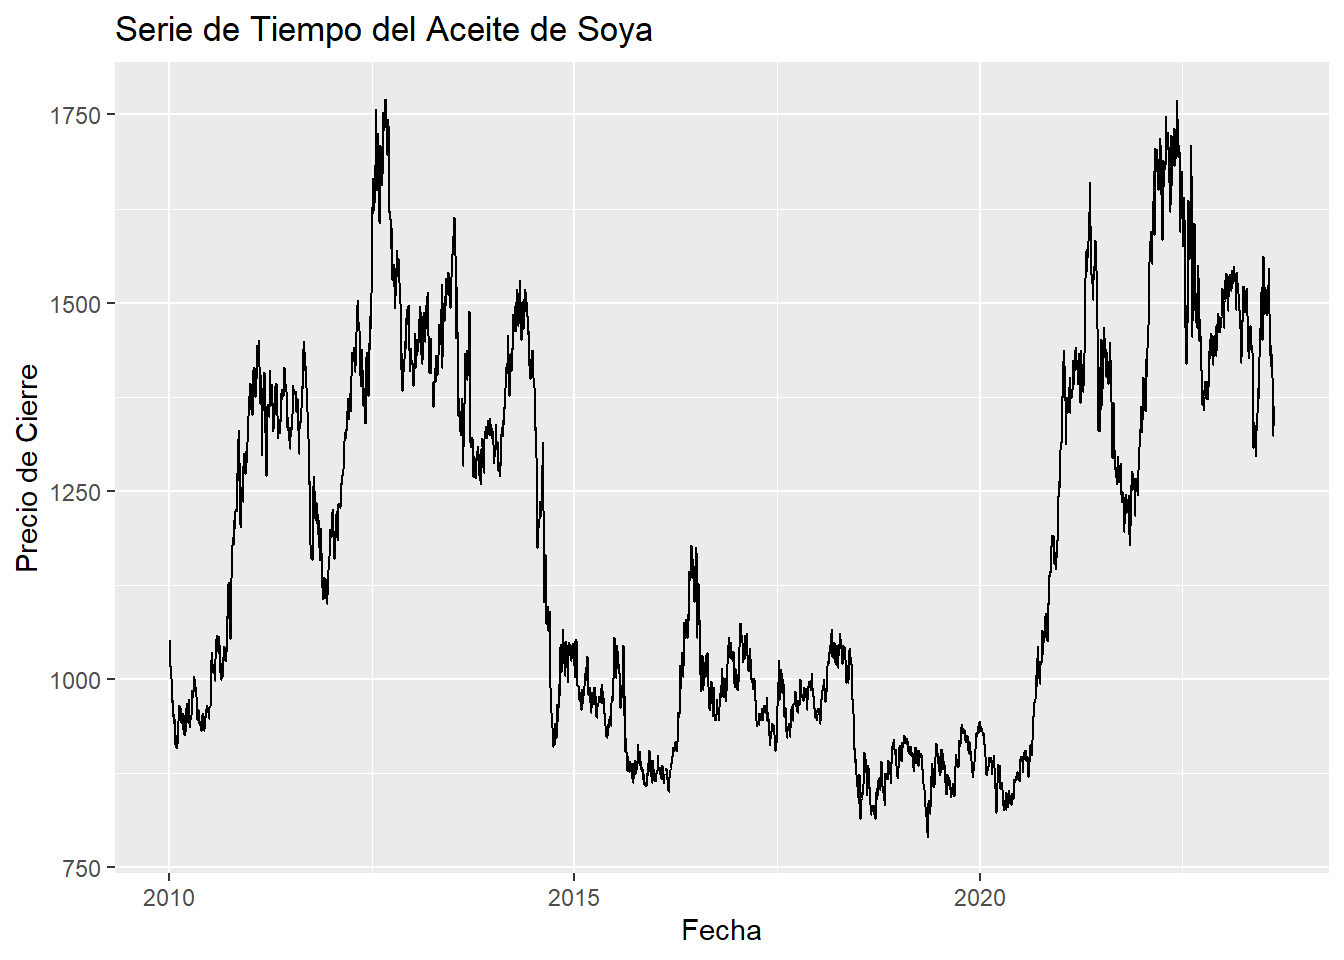
\includegraphics{bookdown-demo_files/figure-latex/unnamed-chunk-2-1.pdf}

\hypertarget{promedio-movil--rezago-y-estacionalidad}{%
\chapter{Promedio Movil- Rezago y Estacionalidad}\label{promedio-movil--rezago-y-estacionalidad}}

Calculamos el promedio móvil simple usando una ventana de 30 días.Introducimos un rezago (lag) a la serie de tiempo.Obtenemos un promedio móvil centrado de 12 meses, suponiendo que la serie tiene estacionalidad anual (común con datos mensuales).

\begin{Shaded}
\begin{Highlighting}[]
\CommentTok{\# Cargar las librerías necesarias}
\FunctionTok{library}\NormalTok{(quantmod)}
\FunctionTok{library}\NormalTok{(dplyr)}
\end{Highlighting}
\end{Shaded}

\begin{verbatim}
## Warning: package 'dplyr' was built under R version 4.2.3
\end{verbatim}

\begin{verbatim}
## 
## ######################### Warning from 'xts' package ##########################
## #                                                                             #
## # The dplyr lag() function breaks how base R's lag() function is supposed to  #
## # work, which breaks lag(my_xts). Calls to lag(my_xts) that you type or       #
## # source() into this session won't work correctly.                            #
## #                                                                             #
## # Use stats::lag() to make sure you're not using dplyr::lag(), or you can add #
## # conflictRules('dplyr', exclude = 'lag') to your .Rprofile to stop           #
## # dplyr from breaking base R's lag() function.                                #
## #                                                                             #
## # Code in packages is not affected. It's protected by R's namespace mechanism #
## # Set `options(xts.warn_dplyr_breaks_lag = FALSE)` to suppress this warning.  #
## #                                                                             #
## ###############################################################################
\end{verbatim}

\begin{verbatim}
## 
## Attaching package: 'dplyr'
\end{verbatim}

\begin{verbatim}
## The following objects are masked from 'package:xts':
## 
##     first, last
\end{verbatim}

\begin{verbatim}
## The following objects are masked from 'package:stats':
## 
##     filter, lag
\end{verbatim}

\begin{verbatim}
## The following objects are masked from 'package:base':
## 
##     intersect, setdiff, setequal, union
\end{verbatim}

\begin{Shaded}
\begin{Highlighting}[]
\FunctionTok{library}\NormalTok{(ggplot2)}
\FunctionTok{library}\NormalTok{(zoo)}

\CommentTok{\# Simbolo del aceite de soya en Yahoo Finance}
\NormalTok{company }\OtherTok{\textless{}{-}} \StringTok{\textquotesingle{}ZS=F\textquotesingle{}}

\CommentTok{\# Definir fecha de inicio y del día de hoy}
\NormalTok{start }\OtherTok{\textless{}{-}} \FunctionTok{as.Date}\NormalTok{(}\StringTok{"2010{-}01{-}01"}\NormalTok{)}
\NormalTok{today }\OtherTok{\textless{}{-}} \FunctionTok{Sys.Date}\NormalTok{()}

\CommentTok{\# Conexión a Yahoo Finance para descargar la información}
\NormalTok{df }\OtherTok{\textless{}{-}} \FunctionTok{getSymbols}\NormalTok{(company, }\AttributeTok{src =} \StringTok{"yahoo"}\NormalTok{, }\AttributeTok{from =}\NormalTok{ start, }\AttributeTok{to =}\NormalTok{ today, }\AttributeTok{auto.assign =} \ConstantTok{FALSE}\NormalTok{)}
\end{Highlighting}
\end{Shaded}

\begin{verbatim}
## Warning: ZS=F contains missing values. Some functions will not work if objects
## contain missing values in the middle of the series. Consider using na.omit(),
## na.approx(), na.fill(), etc to remove or replace them.
\end{verbatim}

\begin{Shaded}
\begin{Highlighting}[]
\CommentTok{\# Convertir el objeto xts a un dataframe para usarlo con dplyr y ggplot2}
\NormalTok{df }\OtherTok{\textless{}{-}} \FunctionTok{data.frame}\NormalTok{(}\AttributeTok{Date =} \FunctionTok{index}\NormalTok{(df), }\FunctionTok{coredata}\NormalTok{(df))}

\CommentTok{\# Calcular el promedio móvil de 30 días usando el nombre correcto de la columna}
\NormalTok{df }\OtherTok{\textless{}{-}}\NormalTok{ df }\SpecialCharTok{\%\textgreater{}\%}
  \FunctionTok{mutate}\NormalTok{(}\AttributeTok{MA\_30 =} \FunctionTok{rollmean}\NormalTok{(}\StringTok{\textasciigrave{}}\AttributeTok{ZS.F.Close}\StringTok{\textasciigrave{}}\NormalTok{, }\AttributeTok{k =} \DecValTok{30}\NormalTok{, }\AttributeTok{fill =} \ConstantTok{NA}\NormalTok{, }\AttributeTok{align =} \StringTok{"right"}\NormalTok{))}

\CommentTok{\# Introducir un rezago (por ejemplo, un lag de 1 día)}
\NormalTok{df }\OtherTok{\textless{}{-}}\NormalTok{ df }\SpecialCharTok{\%\textgreater{}\%}
  \FunctionTok{mutate}\NormalTok{(}\AttributeTok{Lag\_1 =} \FunctionTok{lag}\NormalTok{(}\StringTok{\textasciigrave{}}\AttributeTok{ZS.F.Close}\StringTok{\textasciigrave{}}\NormalTok{, }\AttributeTok{n =} \DecValTok{1}\NormalTok{))}

\CommentTok{\# Calcular un promedio móvil centrado de 12 meses (útil para datos mensuales)}
\NormalTok{df }\OtherTok{\textless{}{-}}\NormalTok{ df }\SpecialCharTok{\%\textgreater{}\%}
  \FunctionTok{mutate}\NormalTok{(}\AttributeTok{MA\_12 =} \FunctionTok{rollmean}\NormalTok{(}\StringTok{\textasciigrave{}}\AttributeTok{ZS.F.Close}\StringTok{\textasciigrave{}}\NormalTok{, }\AttributeTok{k =} \DecValTok{12}\NormalTok{, }\AttributeTok{fill =} \ConstantTok{NA}\NormalTok{, }\AttributeTok{align =} \StringTok{"center"}\NormalTok{))}

\CommentTok{\# Gráfica del precio de cierre, promedio móvil de 30 días y promedio móvil centrado de 12 meses}
\FunctionTok{ggplot}\NormalTok{(df, }\FunctionTok{aes}\NormalTok{(}\AttributeTok{x =}\NormalTok{ Date)) }\SpecialCharTok{+}
  \FunctionTok{geom\_line}\NormalTok{(}\FunctionTok{aes}\NormalTok{(}\AttributeTok{y =} \StringTok{\textasciigrave{}}\AttributeTok{ZS.F.Close}\StringTok{\textasciigrave{}}\NormalTok{, }\AttributeTok{color =} \StringTok{"Precio de Cierre"}\NormalTok{)) }\SpecialCharTok{+}
  \FunctionTok{geom\_line}\NormalTok{(}\FunctionTok{aes}\NormalTok{(}\AttributeTok{y =}\NormalTok{ MA\_30, }\AttributeTok{color =} \StringTok{"Promedio Móvil 30 días"}\NormalTok{), }\AttributeTok{na.rm =} \ConstantTok{TRUE}\NormalTok{) }\SpecialCharTok{+}
  \FunctionTok{geom\_line}\NormalTok{(}\FunctionTok{aes}\NormalTok{(}\AttributeTok{y =}\NormalTok{ MA\_12, }\AttributeTok{color =} \StringTok{"Promedio Móvil 12 meses"}\NormalTok{), }\AttributeTok{na.rm =} \ConstantTok{TRUE}\NormalTok{) }\SpecialCharTok{+}
  \FunctionTok{ggtitle}\NormalTok{(}\StringTok{"Serie de Tiempo y Promedios Móviles"}\NormalTok{) }\SpecialCharTok{+}
  \FunctionTok{ylab}\NormalTok{(}\StringTok{"Precio"}\NormalTok{) }\SpecialCharTok{+}
  \FunctionTok{labs}\NormalTok{(}\AttributeTok{color =} \StringTok{"Leyenda"}\NormalTok{) }\SpecialCharTok{+}
  \FunctionTok{theme\_minimal}\NormalTok{()}
\end{Highlighting}
\end{Shaded}

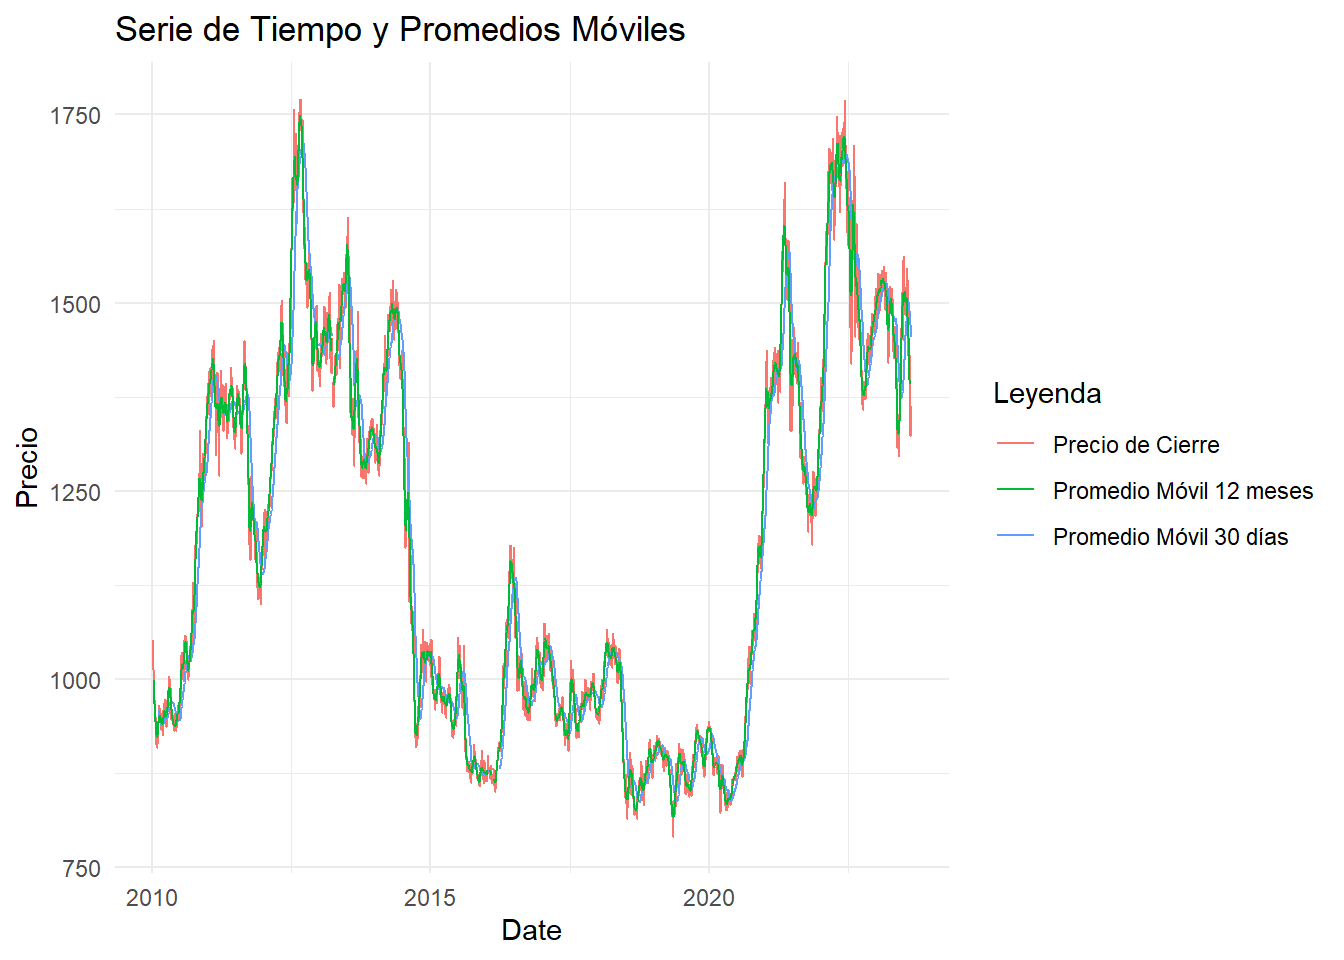
\includegraphics{bookdown-demo_files/figure-latex/unnamed-chunk-3-1.pdf}

\hypertarget{final-words}{%
\chapter{Final Words}\label{final-words}}

We have finished a nice book.

  \bibliography{book.bib,packages.bib}

\end{document}
